\documentclass[12pt]{article}
\usepackage{url,graphicx,tabularx,array,geometry}
\usepackage{listings}
\usepackage[utf8]{inputenc}
\usepackage{setspace}
\usepackage{amsmath}
\usepackage{enumitem}
\setlength{\parskip}{1ex} %--skip lines between paragraphs
\setlength{\parindent}{0pt} %--don't indent paragraphs

%-- Commands for header
\renewcommand{\title}[1]{\textbf{#1}\\}
\renewcommand{\line}{\begin{tabularx}{\textwidth}{X>{\raggedleft}X}\hline\\\end{tabularx}\\[-0.5cm]}
\newcommand{\leftright}[2]{\begin{tabularx}{\textwidth}{X>{\raggedleft}X}#1%
& #2\\\end{tabularx}\\[-0.5cm]}

\onehalfspacing
%\linespread{2} %-- Uncomment for Double Space
\begin{document}

\title{Imperative and System Programming Autumn 2013}
\line
\leftright{\today}{Alexander Rüedlinger, 08-129-710, Group 05} %-- left and right positions in the header
\section*{Series 4}
\subsection*{Stack light basic}
\paragraph{a)} 
\emph{Behaviour:}
By removing an element from an empty stack the test program STACK\_test\_BA terminates with an EXIT FAILURE return value. On posix system this value is 1 and is defined in the header file stdlib.h and indicates the os that a error occurred.

The implementation of the stack has a max capacity of four elements. By pishing fourth element on the stack the test program terminates with an EXIT FAILURE return value.

\emph{Implementation:}
According the stack implementation the behaviour of the test program by removing an element from an empty stack is correct. The variable top "points" to next free place in the int array base. If top points to zero and get is called the stack implementation terminates with an EXIT FAILURE.

If the variable top "points" on the position after the last valid place in the stack (index 4) it terminates with an EXIT FAILURE.

In all cases the test program behaves according the stack implementation.

\paragraph{b)}
The C bible (KR, page 85) states that in the absence of explicit initialization, external and static variables are guaranteed to be initialized to zero. Automatic and register variables have undefined initial values, that is garbage values.

Because the variable top is a external and static variable it is implicit initialized to zero.

The code should be clear, understandable and maintainable therefore it is better to initialize variables explicit form a programmers perspective.

\paragraph{c)}
The variable top and the array base are declared static, because they are used as glocal permanent storage. Because the variable is declared outside the main function top and the base array are global variables which are accessible by all functions declared in the same source code file. But the static keyword makes both global variables only local accessible in the file which they're defined. So their global scope is limited which is referred as glocal.
This protects the variable base and top to be modified by "strangers" or by other programs and eliminates the possibility of side effects. 

\paragraph{d)}
The error states that the variable base is modified at file scope.
An answer on stackoverflow.com related to this problem says that the keyword const doesn't mean a constant in C. It means "read only". Therefore the value CAPACITY which is stored at a memory address could be changed by machine code.

\paragraph{e)}
\begin{lstlisting}
#define CAPACITY 4
\end{lstlisting}

The symbolic constants is preprocessed by the c preprocessor. Each occurrence of this string is replaced by its definition. The C bible says that the scope of symbolic constants is from its point of definition to the end of the source file being compiled.

In case (1) the symbolic constants CAPACITY is placed inside a header file. Here the scope starts with the first file that includes the header file STACK\_SR\_Specif.h and ends until the file is being compiled.

In case (3) the scope of CAPACITY starts from the point of its definition until the file is being compiled.

If we move the symbolic constants into the header file then the macro CAPACITY becomes part of the stack specification. One disadvantage is that the capacity detail is exposed in the header file which is a kind of a "interface". An advantage is that the capacity can easily be in the header file specification and not in the implementation. 

Life time does not make any sense because a macro is not a variable it is just a text replacement performed by the preprocessor. But it makes sense to think about the scope of a macro which is global.

\paragraph{f)}

In the java programming language such a procdure is called peek in the stack interface:\\ 
\url{http://docs.oracle.com/javase/7/docs/api/java/util/Stack.html#peek()}

Thus I name this procedure stack\_peek() to retrieve the top value of the stack.
The following listing shows the implementation:
\begin{lstlisting}
int stack_peek(){
	if(top == 0) exit(EXIT_FAILURE);
	return base[top-1];
}
\end{lstlisting}

Besides that I put a prototype in the header file STACK\_SR\_Specif.h and i adapted the STACK\_test.c file to test the peek function.
\subsection*{Scope and Lifetime}
Nothing todo.

\subsection*{Make: A First Contact}

\paragraph{Question 1)} Draw the dependency tree of hello.
Content of the makefile in the hello example:
\begin{lstlisting}
hello : hello.o tellMe.o
	gcc -o hello hello.o tellMe.o
hello.o : hello.c
	gcc -c hello.c
tellMe.o : tellMe.c
	gcc -c tellMe.c

clean:
	rm hello.o tellMe.o hello
\end{lstlisting}

\begin{figure}[!htb]
\centering
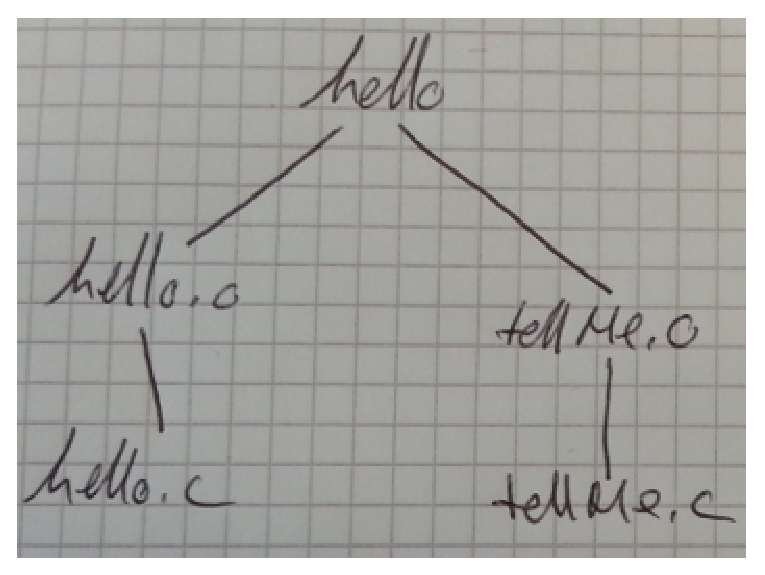
\includegraphics[scale=0.5]{make_dep_q1.eps} 
\caption{Dependencies of hello}
\end{figure}

\paragraph{Q2)}
\begin{lstlisting}
(1) make
(2) touch tellMe.c   # or modify (3) tellMe.c
(4) make tellMe.o
(5) make
(6) make             # sic!, redo a (7) make
(8) make -W tellMe.c
\end{lstlisting}

The first command just executes the Makefile in the directory.
The output is as follows:
\begin{lstlisting}
gcc -c hello.c
gcc -c tellMe.c
gcc -o hello hello.o tellMe.o
\end{lstlisting}
Because these files were not compiled before, the whole dependency tree has been compiled.
Overall the output says that hello.c and tellMe.c

The second command touch just modifies the unix timestamp of the file tellMe.c 
More precisly the man page says it changes file access and modification times.

Before I execute touch tellMe.c

I perform a ls -ltr:
\begin{lstlisting}
$ ls -ltr
total 32
-rwx------ 1 lexruee lexruee   39 Apr 18  2005 hello.c
-rwx------ 1 lexruee lexruee   55 Apr 18  2005 tellMe.c
-rwx------ 1 lexruee lexruee  162 Mar 12  2008 Makefile
-rw-rw-r-- 1 lexruee lexruee 1352 Oct 15 09:24 hello.o
-rw-rw-r-- 1 lexruee lexruee 1488 Oct 15 09:24 tellMe.o
-rwxrwxr-x 1 lexruee lexruee 8583 Oct 15 09:24 hello
\end{lstlisting}
The command ls -ltr shows the directory in a long listing format and it shows the modification time of each file. So last time tellMe.c was modified dates back in Apr 18  2005.

After I execute touch tellMe.c I get the output:
\begin{lstlisting}
$ ls -ltr
total 32
-rwx------ 1 lexruee lexruee   39 Apr 18  2005 hello.c
-rwx------ 1 lexruee lexruee  162 Mar 12  2008 Makefile
-rw-rw-r-- 1 lexruee lexruee 1352 Oct 15 09:24 hello.o
-rw-rw-r-- 1 lexruee lexruee 1488 Oct 15 09:24 tellMe.o
-rwxrwxr-x 1 lexruee lexruee 8583 Oct 15 09:24 hello
-rwx------ 1 lexruee lexruee   55 Oct 15 09:40 tellMe.c
\end{lstlisting}
Indeed the command touch has changed the access and modification time to Oct 15 09:40.

The third line make tellMe.o updates the target tellMe.o. It compiles the source file tellMe.c again, that's because we've changed the modification time.

The line produces the output:
\begin{lstlisting}
$ make tellMe.o
gcc -c tellMe.c
\end{lstlisting}

As said before it compiles the dependency tellMe.c of the target tellMe.o again. This makes absolutely sense because by the command touch we have changed the modification time and make has noticed this.

The fourth command make just executes again the file Makefile in the directory. Because the target tellMe.o has been changed the other targets will be updated. But because the target hello.o has not be changed no further files are compiled.

The output is given as follows:
\begin{lstlisting}
$ make
gcc -o hello hello.o tellMe.o
\end{lstlisting}

Here we can see that make wants to update the dependencies hello.o and tellMe.o.
As we can see no actions are performed because no changes have been made.

In the fifth line make is again executed. As mentioned before nothing will happen, because the unix timestamps of the files have not been changed. 

So the output is:
\begin{lstlisting}
$ make
make: `hello' is up to date.
\end{lstlisting}

As the output states all dependencies are fresh.

The last line make -W tellMe.c pretends that the file tellMe.c has been modified. It shows what would happen if we change the file tellMe.c. 

It would compile tellMe.c and it would update the targets hello. and tellMe.o.

\begin{lstlisting}
$ make -W tellMe.c
gcc -c tellMe.c
gcc -o hello hello.o tellMe.o
\end{lstlisting}

This is exactly in line with what we've mentioned above.


\paragraph{Q3)}

Figure for (1)

\begin{figure}[!htb]
\centering
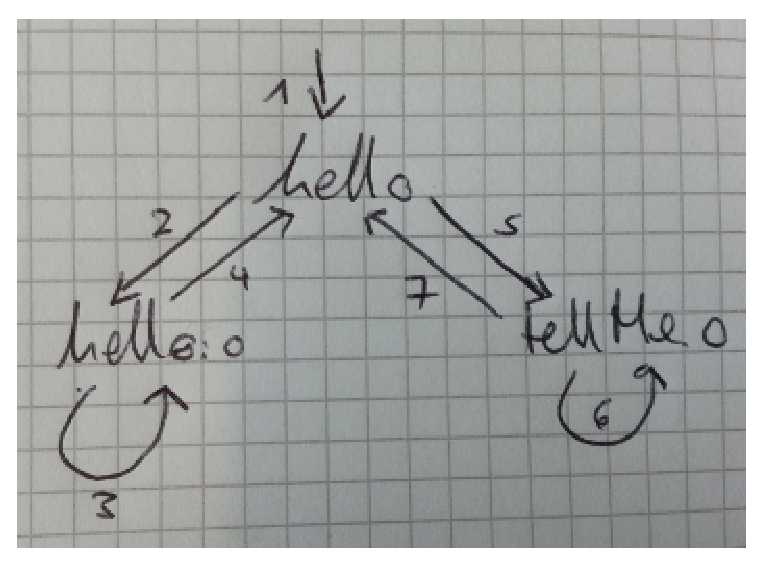
\includegraphics[scale=0.5]{make_dep_q3_1.eps} 
\caption{(1) dependency tree}
\end{figure}

Figure for (3)

\begin{figure}[!htb]
\centering
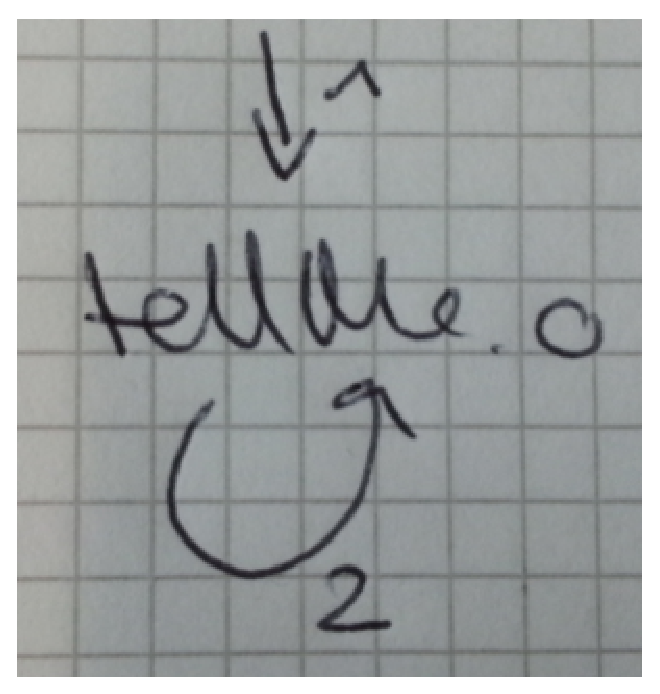
\includegraphics[scale=0.5]{make_dep_q3_2.eps} 
\caption{(3) dependency tree}
\end{figure}

Figure for 4)

\begin{figure}
\centering
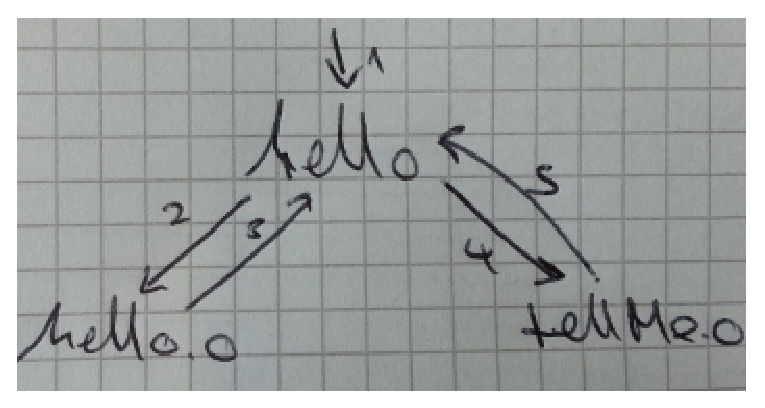
\includegraphics[scale=0.5]{make_dep_q3_4.eps} 
\caption{4) dependency tree}
\end{figure}


Figure for 5)

\begin{figure}[!htb]
\centering
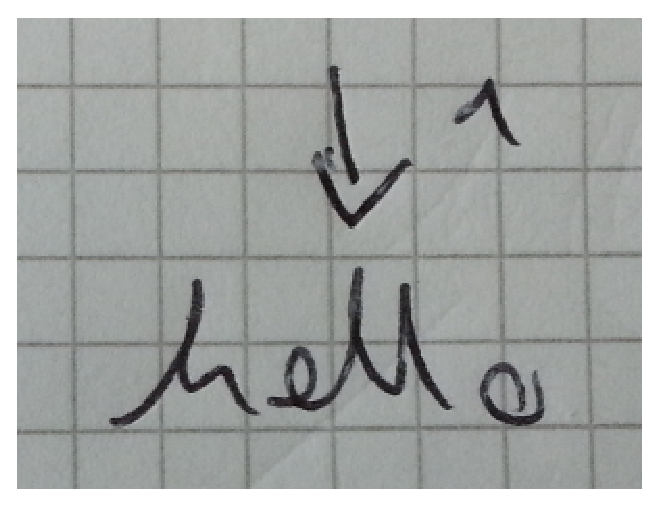
\includegraphics[scale=0.5]{make_dep_q3_5.eps} 
\caption{5) dependency tree}
\end{figure}

Figure for 6)

\begin{figure}[!htb]
\centering
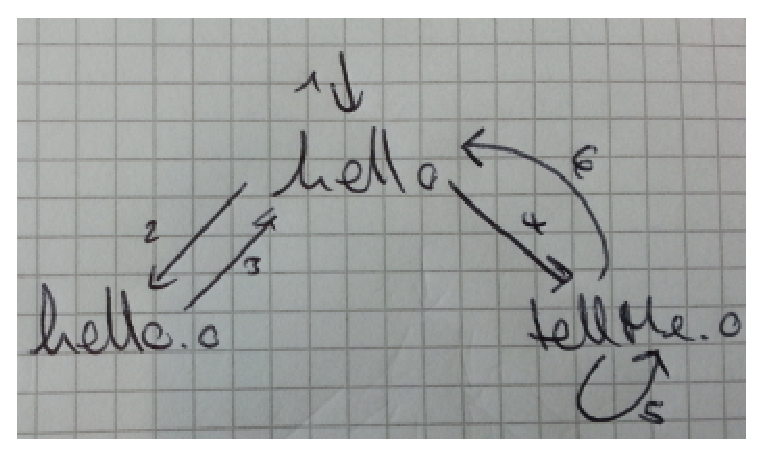
\includegraphics[scale=0.5]{make_dep_q3_6.eps} 
\caption{6) dependency tree}
\end{figure}

\subsubsection*{Header Files: Hello World (revisited)}
Running make on the terminal to compile all four programs yields to:
\begin{lstlisting}
$ make
gcc -c hello.c
gcc -c tellMe.c
gcc -o hello hello.o tellMe.o
gcc -c tellMe\_unwiseBug.c
gcc -o hello\_unwiseBug hello.o tellMe\_unwiseBug.o
gcc -c tellMe\_execBug.c
gcc -o hello\_execBug hello.o tellMe\_execBug.o
gcc -c tellMe\_compBug.c
tellMe\_compBug.c:7:6: error: conflicting types for tellMe
In file included from tellMe\_compBug.c:5:0:
tellMe.h:1:6: note: previous declaration of tellMe was here
make: *** [tellMe\_compBug.o] Error 1
lexruee@death-star:~/unifr\_workspace/ip/homeworks/series\_4/Makefile Examples/2.
\end{lstlisting}
In the file tellMe\_compBug.c we encounter a compile time error.
As a result we've three programs that were successfully compiled (all except for X\_comBug.c).


The program hello produces the output:
\begin{lstlisting}
$./hello

   tellMe> Hello World
\end{lstlisting}

This program behaves correctly and contains no bug. That's because tellMe.c implements the specification tellMe.h correctly!


The program hello\_execBug produces the output:
\begin{lstlisting}
$ ./hello_execBug 

   tellMe> 100

   tellMe> execution BUG !!!
\end{lstlisting}
This programs has in the prototype tellMe only a character as parameter and not an array of characters. Because the program hello.c passes a character array to the function tellMe() the specified function X\_execBug.c copies the address of the passed character array and prints the memory address as decimal number.
Because the header file is not included no type checking is performed. Therefore it compiles.
Otherwise we would have a compile time error like in the file X\_compBug.c


The program hello\_unwiseBug produces the output:
\begin{lstlisting}
$ ./hello_unwiseBug 

   tellMe> Hello World

   tellMe> unwise BUG !!!
\end{lstlisting}

Here the prototype is identical to tellMe.h Therefore the program behaves correctly, but it's prone to become buggy as soon the prototype changes or the type of the passed variable changes.
Here we have the same problem. The c compiler does not perform type checking because of the missing header file. Otherwise we would have a compile time error like in the file X\_compBug.c.

Summarized: Only the program tellMe.c implements the header file tellMe.h in a correct way.


\subsubsection*{Make and Timestamp: about virtually and really retarding the clock}
Running make yields to:
\begin{lstlisting}
$ make
gcc -o hello hello.c
\end{lstlisting}

We run ./hello:
\begin{lstlisting}
$ ./hello
hello
\end{lstlisting}

After compiling hello.c and cp hello.c hello\_old.c I use the command ls -lc to get a list of all files with a timestamp :

\begin{lstlisting}
$ ls -cl
total 24
-rwxrwxr-x 1 lexruee lexruee 8519 Oct 15 13:14 hello
-rwx------ 1 lexruee lexruee   48 Oct 15 09:10 hello.c
-rwx------ 1 lexruee lexruee   48 Oct 15 13:15 hello\_old.c
-rwx------ 1 lexruee lexruee   56 Oct 15 09:10 Makefile
\end{lstlisting}
As we can see both files have not the same timestamp. That's because that hello\_old.c has just been created or copied.

Again we run make:
\begin{lstlisting}
$ make
gcc -o hello hello.c
\end{lstlisting}

Now we look at the timestamps:

\begin{lstlisting}
p$ ls -cl
total 28
-rwxrwxr-x 1 lexruee lexruee 8519 Oct 15 13:22 hello
-rwx------ 1 lexruee lexruee   54 Oct 15 13:22 hello.c
-rwx------ 1 lexruee lexruee   48 Oct 15 13:22 hello.c~
-rwx------ 1 lexruee lexruee   48 Oct 15 13:15 hello_old.c
-rwx------ 1 lexruee lexruee   56 Oct 15 09:10 Makefile
\end{lstlisting}
As we can see the timestamp of hello.c has changed.

After mv hello\_old.c to hello.c:
\begin{lstlisting}
$ ls -cl
total 28
-rwxrwxr-x 1 lexruee lexruee 8519 Oct 15 13:22 hello
-rwx------ 1 lexruee lexruee   54 Oct 15 13:22 hello.c
-rwx------ 1 lexruee lexruee   48 Oct 15 13:22 hello.c~
-rwx------ 1 lexruee lexruee   48 Oct 15 13:15 hello_old.c
-rwx------ 1 lexruee lexruee   56 Oct 15 09:10 Makefile
\end{lstlisting}
Interesting. The renamed file hello\_old.c takes over the timestamp of file hello.c

After running mahe we get:
\begin{lstlisting}
$ make
make: `hello' is up to date.
\end{lstlisting}
So the file hello is update to date and is not compiled although its not the original file!

After running touch hello.c we run again make:
\begin{lstlisting}
make
gcc -o hello hello.c
\end{lstlisting}
Because the command set the current timestamp in hello.c make compiles it again.



\subsection*{Macros and Preprocessor: A First Contact}
\paragraph{Exercise 1)}

Content of pp.txt
\begin{lstlisting}
#define max(A, B) ((A) > (B) ? (A) : (B))
#define square(x) x * x
max(a, b);
max(a+1, b+1);
square(x);
square(x+1);
\end{lstlsiting}

\paragraph{Exercise 1)}

Running the preprocessor on the file pp.txt via:
\begin{lstlisting}
cpp pp.txt
\end{lstlisting}

It produces the following output:
\begin{lstlisting}
# 1 "pp.txt"
# 1 "<command-line>"
# 1 "pp.txt"


((a) > (b) ? (a) : (b));
((a+1) > (b+1) ? (a+1) : (b+1));
x * x;
x+1 * x+1;
\end{lstlisting}

As we can see we should use parentheses around the expression x.
So we should adapt the line 
\begin{lstlisting}
#define square(x) x * x
\end{lstlisting}

into the following line in pp.txt:

\begin{lstlisting}
#define square(x) (x) * (x)
\end{lstlisting}
So this is the correct square macro!

So running cpp on the fixed version of pp.txt yields:
\begin{lstlisting}
# 1 "pp.txt"
# 1 "<command-line>"
# 1 "pp.txt"


((a) > (b) ? (a) : (b));
((a+1) > (b+1) ? (a+1) : (b+1));
(x) * (x);
(x+1) * (x+1);
\end{lstlisting}


\paragraph{Exercise 2)}

My solutions is as follows:
\begin{lstlisting}
#include<stdio.h>
#define swap(int,a,b) a=a^b; b=a^b; a=a^b
main(){
	int a=1, b=2;
	swap(int,a,b);
	printf("%d %d\n", a, b);
}
\end{lstlisting}
We can use the XOR operator to swap the variables without a temporary variable.
That's a nice trick to avoid a third temporary variable ;-)!

On my machine I obtain the following output:
\begin{lstlisting}
 ./swap.o 
2 1
\end{lstlisting}
So the variable were successfully swapped!

\paragraph{Exercise 3)}
a)
Once the macro has be expanded we have the following source file:
\begin{lstlisting}
#include<stdio.h>
main(){
	int a=1, b=2;
	if(a>b)
	     a=a^b; 
	b=a^b; 
	a=a^b;
	else a = b;
	printf("%d %d\n", a, b);
}
\end{lstlisting}

This is invalid c code. Because after the if statement without curly braces only one statement must occur if a else statement follows.
b)
\begin{lstlisting}
#include<stdio.h>
#define swap(int,a,b)  a=a^b,b=a^b,a=a^b
main(){
	int a=1, b=2;
	if (a>b) swap(int,a,b);
	else a = b;
	printf("%d %d\n", a, b);
}
\end{lstlisting}

This solution is correct and produces valid c code.

\subsection*{Process Memory Model}
Nothing todo.

\end{document}